\documentclass[a4paper, oneside]{article}

\makeatletter
    \renewcommand\paragraph{%
        \@startsection{paragraph}{4}{0mm}%
           {-\baselineskip}%
           {.5\baselineskip}%
           {\normalfont\normalsize\bfseries}}
    \makeatother


\usepackage{../../Stile/mercuryseven}
\usepackage{titlesec}
\newcommand{\Titolo}{Piano Di Progetto}

\newcommand{\VersioneDocumento}{\versPdP}

\newcommand{\ACapoRedazione}{\textit{\Davide{}} \newline \textit{\Francesco{}} \newline{} \textit{\Matteo{}}}

\newcommand{\Verifica}{\textit{\Daniele{}} \newline{} \textit{\Lucrezia{}} \newline{} \textit{\Giosue{}}}

\newcommand{\Responsabile}{\textit{\Tommaso{}}}

\newcommand{\Distribuzione}{\textit{Prof. \Tullio{}} \newline \textit{Prof. \Riccardo{}} \newline Gruppo \textit{\Gruppo{}}}

\newcommand{\Uso}{Esterno}

\newcommand{\DescrizioneDoc}{Descrizione della pianificazione realizzata da \textit{\Gruppo{}}, l'analisi dei rischi che potrebbero verificarsi, il prospetto economico e l'organigramma}

\begin{document}
\copertina{}
\section*{\centerline{Registro delle modifiche}}
{
	\newlength{\freewidth}
	\setlength{\freewidth}{\dimexpr\textwidth-10\tabcolsep}
	\renewcommand{\arraystretch}{1.5}
	\centering
	\setlength{\aboverulesep}{0pt}
	\setlength{\belowrulesep}{0pt}
	\rowcolors{2}{AzzurroGruppo!10}{white}
	\begin{longtable}{C{.131777\freewidth} C{.134036\freewidth} C{.263554\freewidth} C{.188254\freewidth} C{.282379\freewidth}}
		\toprule 
		\rowcolor{AzzurroGruppo!30}
		\textbf{Versione} & \textbf{Data} & \textbf{Autore} & \textbf{Ruolo} & \textbf{Descrizione}\\
		\toprule
		\endhead

		v1.0.0-0.10 & 2021-04-15 & \Matteo{} & \RdP{} & Approvazione del documento. \\
		v0.4.0-0.10 & 2021-04-14 & \Daniele{}, \newline{} \Lucrezia{} & \ver{}, \newline{} \prog{} & Correzione e verifica segnalazioni Product Baseline.\\
		v0.3.0-0.9 & 2021-04-05 & \Daniele{}, \newline{} \Giosue{} & \ver{}, \newline{} \progr{} & Stesura e verifica glossario. \\
		v0.2.1-0.9 & 2021-04-03 & \Davide{}, \newline{} \Lucrezia{} & \ver{}, \newline{} \prog{} & Aggiunta e verifica immagini. \\
		v0.2.0-0.9 & 2021-04-02 & \Davide{}, \newline{} \Giosue{} & \ver{}, \newline{} \progr{} & Stesura e verifica test e archittettura. \\
		v0.1.0-0.9 & 2021-03-30 & \Daniele{}, \newline{} \Giosue{} & \ver{}, \newline{} \progr{} & Stesura e verifica tecnologie e librerie. \\
		v0.0.2-0.9 & 2021-03-26 & \Davide{}, \newline{} \Lucrezia{} & \ver{},\newline{} \prog{} & Stesura e verifica introduzione. \\
		v0.0.1-0.8 & 2021-03-23 & \Davide{},\newline{} \Lucrezia{} & \ver{},\newline{} \prog{} & Stesura e verifica scheletro documento. \\
		\bottomrule
		\hiderowcolors
	\end{longtable}
}
\newpage
\newpage
\tableofcontents
\listoftables
\newpage
\section{Introduzione}
\subsection{Scopo del documento}
Lo scopo di questo documento è illustrare tutte le funzionalità del \gloman{sync engine} richiesto dal capitolato \textit{C7}. L'utente finale, in questo modo, avrà a disposizione tutte le indicazioni per il corretto uso del \gloman{software}.

\subsection{Scopo del prodotto}
Lo scopo del capitolato \textit{C7} è la creazione di un algoritmo \gloman{solido} ed efficiente in grado di garantire il salvataggio e la sincronizzazione dei cambiamenti presenti in \gloman{cloud}. È inoltre richiesta la creazione di una interfaccia grafica multipiattaforma. Il progetto deve dunque funzionare sui principali sistemi operativi desktop quali Windows, macOS e Linux senza richiedere l'installazione manuale di ulteriori prodotti per il corretto funzionamento. 
\subsection{Obiettivo del prodotto}
L'obiettivo del progetto è la realizzazione di un modulo per la piattaforma \gloman{Zimbra}, che abbia le caratteristiche sopra descritte, e che si appoggi per il suo funzionamento al \gloman{cloud} \gloman{Zextras Drive}.
Nello specifico, lo scopo finale del prodotto è quello di fornire agli utenti un servizio che automatizzi il salvataggio e la sincronizzazione con il \gloman{cloud}.
\subsection{Glossario}
Nel documento sono presenti termini che possono presentare dei significati ambigui o poco chiari a seconda del contesto.
Per evitare incomprensioni il gruppo fornisce un glossario individuabile nell'appendice \S{}\ref{sec:Glossario} contenente i termini e la loro spiegazione.\newline{}
Nel documento corrente si è deciso di segnare tutte le parole presenti nel \G{} con una "G" a pedice di ogni parola.
\newpage
\section{Requisiti minimi di sistema}

\subsection{Requisiti hardware}

Non vi sono particolari requisiti minimi per l'utilizzo del \gloman{software}. Vi è da notare comunque che più la cartella da sincronizzare è grande e più il programma richiederà maggiori risorse.

\subsection{Requisiti software}
{
	\setlength{\freewidth}{\dimexpr\textwidth-1\tabcolsep}
	\renewcommand{\arraystretch}{1.5}
	\setlength{\aboverulesep}{0pt}
	\setlength{\belowrulesep}{0pt}
	\rowcolors{2}{AzzurroGruppo!10}{white}
	\begin{longtable}{L{.210\freewidth} C{.68\freewidth}}
		\rowcolor{AzzurroGruppo!30}
		\textbf{Sistema operativo} & \textbf{Versione minima testata} \\
		\toprule
		\endhead
		Windows & 10 \\
		macOS & 11.0 \\
		Ubuntu & 20.10 \\

		\bottomrule
		\hiderowcolors
		\caption{Sistemi operativi supportati}
	\end{longtable}
}

\subsection{Segnalazione bug}

Nel caso si riscontrassero \gloman{bug} o problemi di qualsiasi tipo, preghiamo di segnalarlo al seguente indirizzo email:\newline{}
\centerline{\url{mercuryseven.swe@gmail.com}}
Oppure per utenti più esperti è possibile aprire una issue su \gloman{GitHub} al seguente link:\newline{}
\centerline{\url{https://github.com/MercurySeven/project-SSD}}

\newpage
\section{Installazione ed avvio di SSD}
Per installare ed avviare l'applicazione \gloman{SSD} bisogna effettuare passi diversi in base al sistema operativo. Le varie versioni possono essere scaricate dal link: \newline{}
\centerline{\url{https://github.com/MercurySeven/project-SSD/releases}}

\subsection{Windows}
\begin{itemize}
\item \textbf{Scaricare:} cliccare sull'apposito link e scaricare il file denominato \textit{SSD.exe};
\item \textbf{Avviare l'applicazione:} cliccare sull'applicazione appena scaricata.
\end{itemize}

\subsection{MacOS}
\begin{itemize}
\item \textbf{Scaricare:} cliccare sull'apposito link e scaricare il file denominato \textit{ssdMacOS.zip};
\item \textbf{Avviare l'applicazione:} decomprimere il file, aprire la cartella e cliccare il file \textit{"launch.command"}, premere \textit{consenti} a ogni finestra pop-up che si aprirà.
\end{itemize}

\subsection{Linux}
\begin{itemize}
\item \textbf{Scaricare:} cliccare sull'apposito link e scaricare il file denominato \textit{SSD.AppImage};
\item \textbf{Avviare l'applicazione:} cliccare sull'applicazione appena scaricata.
\end{itemize}


\newpage
\section{Istruzioni per l'utilizzo}

\subsection{Primo avvio}
\subsubsection{Selezione del percorso dove sincronizzare}
\label{sec:selezionepath}
Al primo avvio, verrà chiesto di scegliere una cartella dove verranno salvati i file presenti nel server e dove l'utente inserirà i nuovi file che vorrà sincronizzare.
\begin{figure}[H]
    \centering
    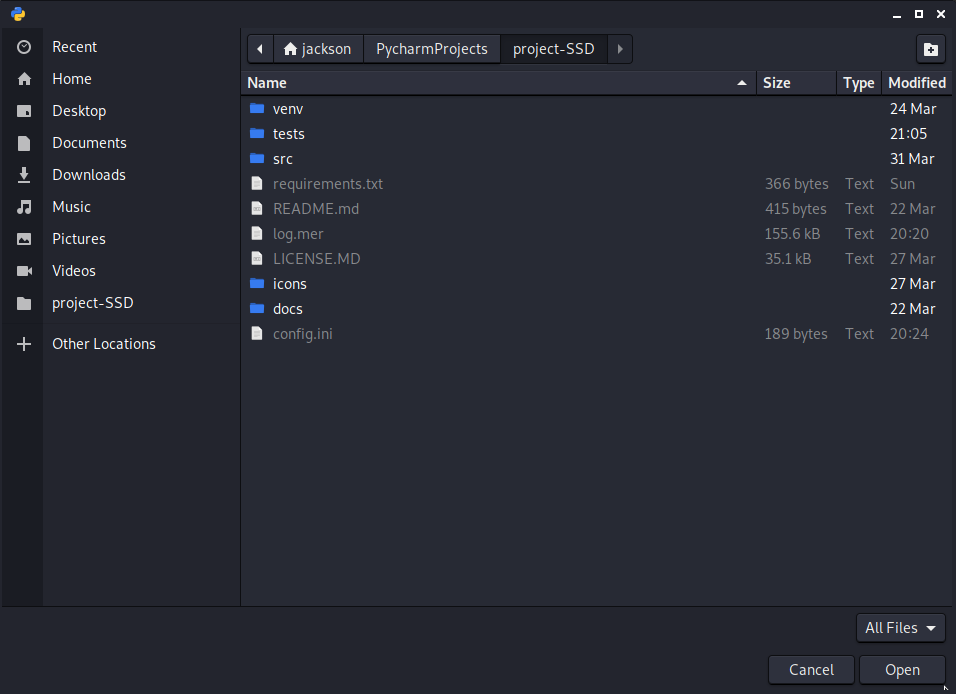
\includegraphics[scale = 0.50]{components/img/selezione-path.png}
    \caption{Selezione del percorso dove sincronizzare}
    \label{fig:Selezione del percorso dove sincronizzare}
\end{figure}


\subsubsection{Autenticazione}
\label{sec:autenticazione}
Successivamente verrà mostrata una form di login, nella quale bisognerà inserire nome utente e password del proprio account \gloman{Zextras Drive} (Fig. \ref{fig:Vista del login}).
Se il login è completato con successo, si avvierà il \gloman{software}, altrimenti verrà visualizzato un messaggio di errore e chiesto di reinserire le credenziali (Fig. \ref{fig:errore login}). \newline
Negli avvii successivi, il login verrà effettuato automaticamente, a meno che non sia stato effettuato il logout (\S{}\ref{sec:profilo}) o la password dell'account sia stata cambiata.
\begin{figure}[H]
    \centering
    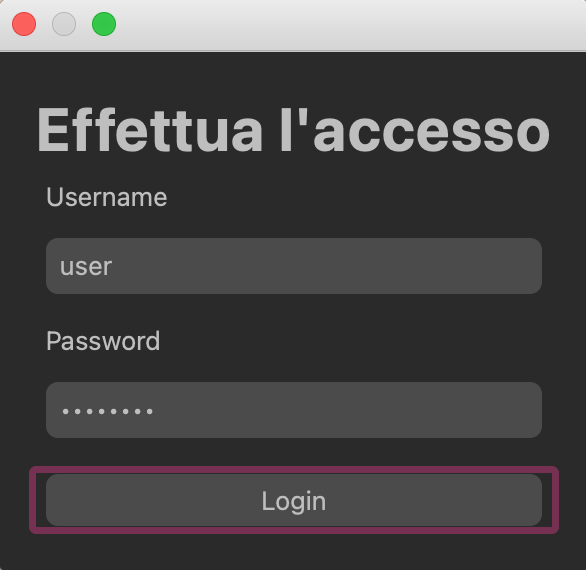
\includegraphics[scale = 0.50]{components/img/login.png}
    \caption{Login}
    \label{fig:Vista del login}
\end{figure}
\begin{figure}[H]
    \centering
    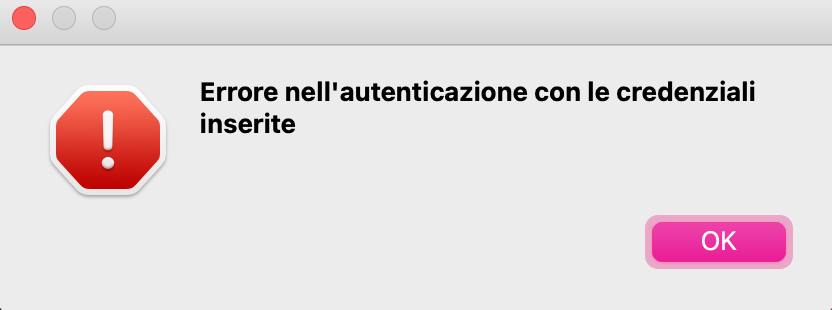
\includegraphics[scale = 0.50]{components/img/err-login.png}
    \caption{Errore di autenticazione}
    \label{fig:errore login}
\end{figure}


\subsection{Finestra principale}
\label{sec:principale}
\begin{figure}[H]
    \centering
    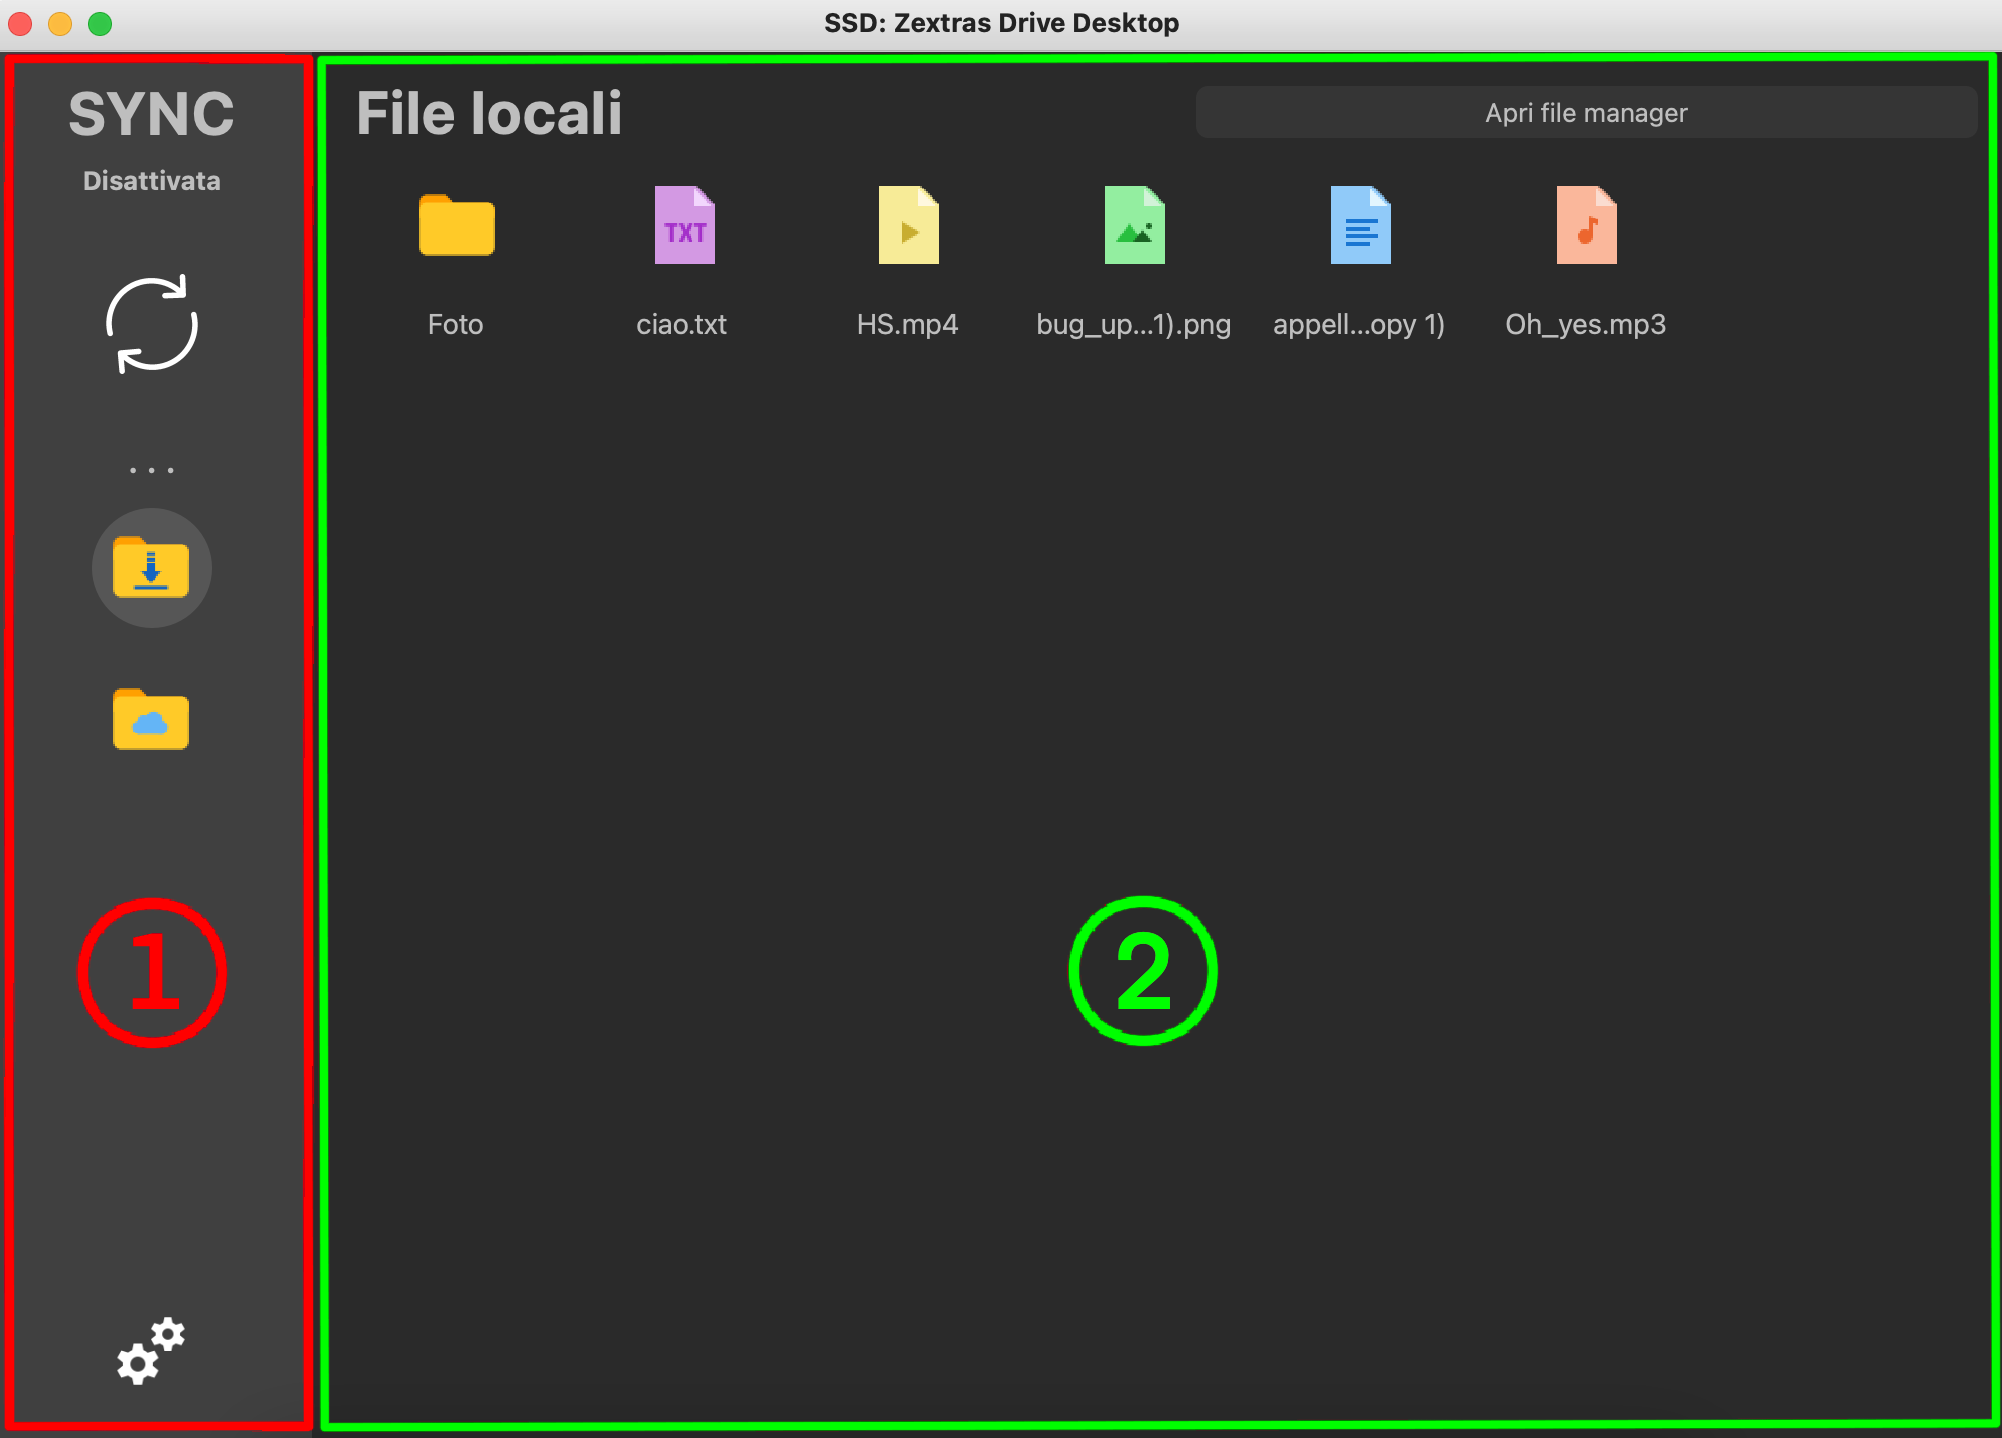
\includegraphics[scale = 0.7]{components/img/Principale.png}
    \caption{Vista schermata principale}
    \label{fig:principale}
\end{figure}
Una volta avviato il software si aprirà una finestra,  mostrata in Fig. \ref{fig:principale}, nella quale verranno visualizzati:
\begin{enumerate}
\item Menù laterale (\S{}\ref{sec:menu});\
\item Finestra principale, che cambia in base al pulsante selezionato nel menù.\
\end{enumerate}


\subsubsection{Menù laterale}
\label{sec:menu}
Il menù laterale è posizionato a sinistra della vista e presenta quattro pulsanti:
\begin{itemize}
\item \textbf{Pulsante di sincronizzazione}: attiva e disattiva la sincronizzazione della cartella locale con il server; \
\end{itemize}
\begin{figure}[H]
\centering
\begin{minipage}[b]{0.45\linewidth}
\centering

\includegraphics[scale=0.5]{components/img/SyncA.png}
\caption{Sincronizzazione attivata}
\label{fig:PsyncA}
\end{minipage}
\quad
\begin{minipage}[b]{0.45\linewidth}
\centering

\includegraphics[scale=0.5]{components/img/SyncD.png}
\caption{Sincronizzazione disattivata}
\label{fig:PsyncD}
\end{minipage}
\end{figure}
\begin{itemize}
\item \textbf{Pulsante file sincronizzati}: mostra la cartella locale sincronizzata (\S{}\ref{sec:fileLocali}); \
\end{itemize}
\begin{figure}[H]
    \centering
    
\includegraphics[scale = 1]{components/img/pulsanteFileS.png}
    \caption{Pulsante file sincronizzati}
    \label{fig:PfileSync}
\end{figure}
\begin{itemize}
\item \textbf{Pulsante file remoti}: mostra i file presenti sul server (\S{}\ref{sec:fileRemoti}); \
\end{itemize}
\begin{figure}[H]
    \centering
    
\includegraphics[scale = 1]{components/img/pulsanteFileR.png}
    \caption{Pulsante file remoti}
    \label{fig:PfileRem}
\end{figure}
\begin{itemize}
\item \textbf{Pulsante delle impostazioni}: mostra le impostazioni del software (\S{}\ref{sec:impostazioni}). \
\end{itemize}
\begin{figure}[H]
    \centering
    
\includegraphics[scale = 1]{components/img/pulsanteImpostazioni.png}
    \caption{Pulsante impostazioni}
    \label{fig:PImp}
\end{figure}


\subsection{File locali}
\label{sec:fileLocali}
\begin{figure}[H]
    \centering
    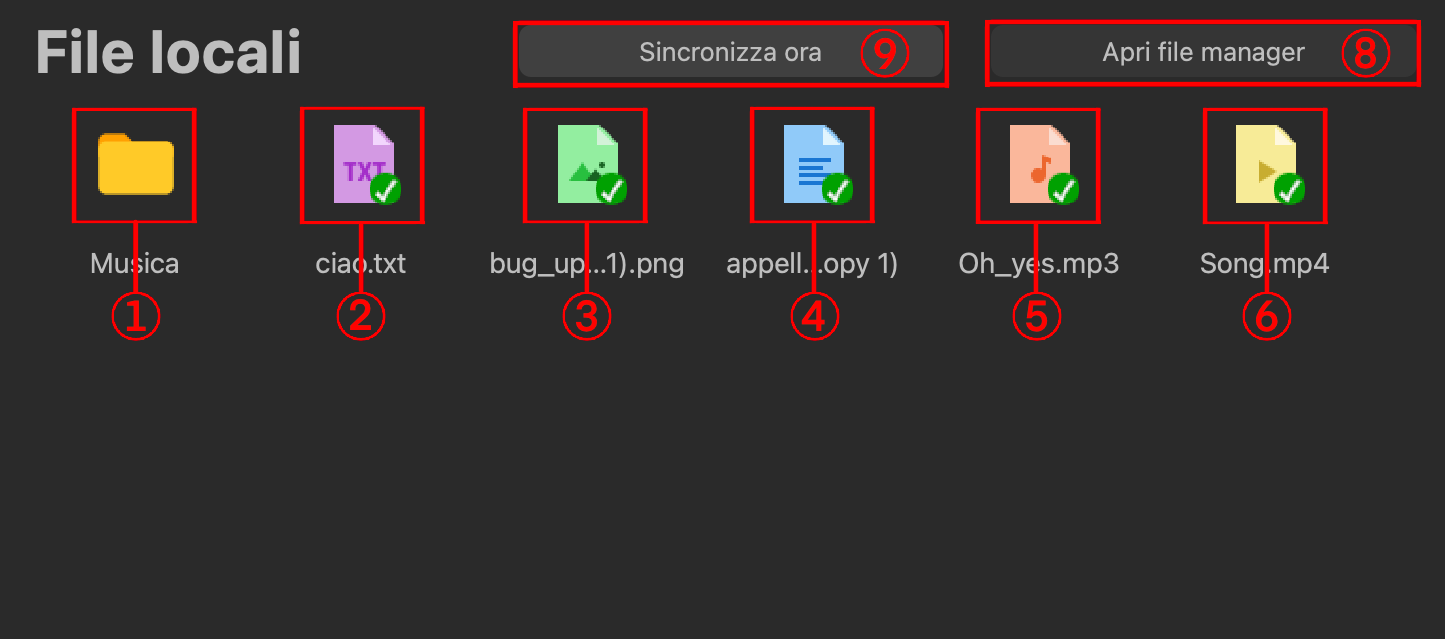
\includegraphics[scale = 0.9]{components/img/fileLocali.png}
    \caption{Vista file locali}
    \label{fig:fileSync}
\end{figure}
La vista si compone di una serie di icone che rappresentano i file o le cartelle presenti nella cartella condivisa. Le icone possono rappresentare:
\begin{itemize}
\item \textbf{Cartella [1]};\
\item \textbf{File di testo [2]};\
\item \textbf{File immagine [3]};\
\item \textbf{File generico [4]};\
\item \textbf{File audio [5]};\
\item \textbf{File video [6]}.\
\end{itemize}
In alto a destra ci sono due pulsanti:
\begin{itemize}
\item \textbf{Sincronizza ora [7]}: permette di forzare la sincronizzazione con il server;\
\item \textbf{Apri file manager [8]}: apre la cartella rappresentata tramite il file manager del computer.\
\end{itemize}


\subsection{File remoti}
\label{sec:fileRemoti}
\begin{figure}[H]
    \centering
    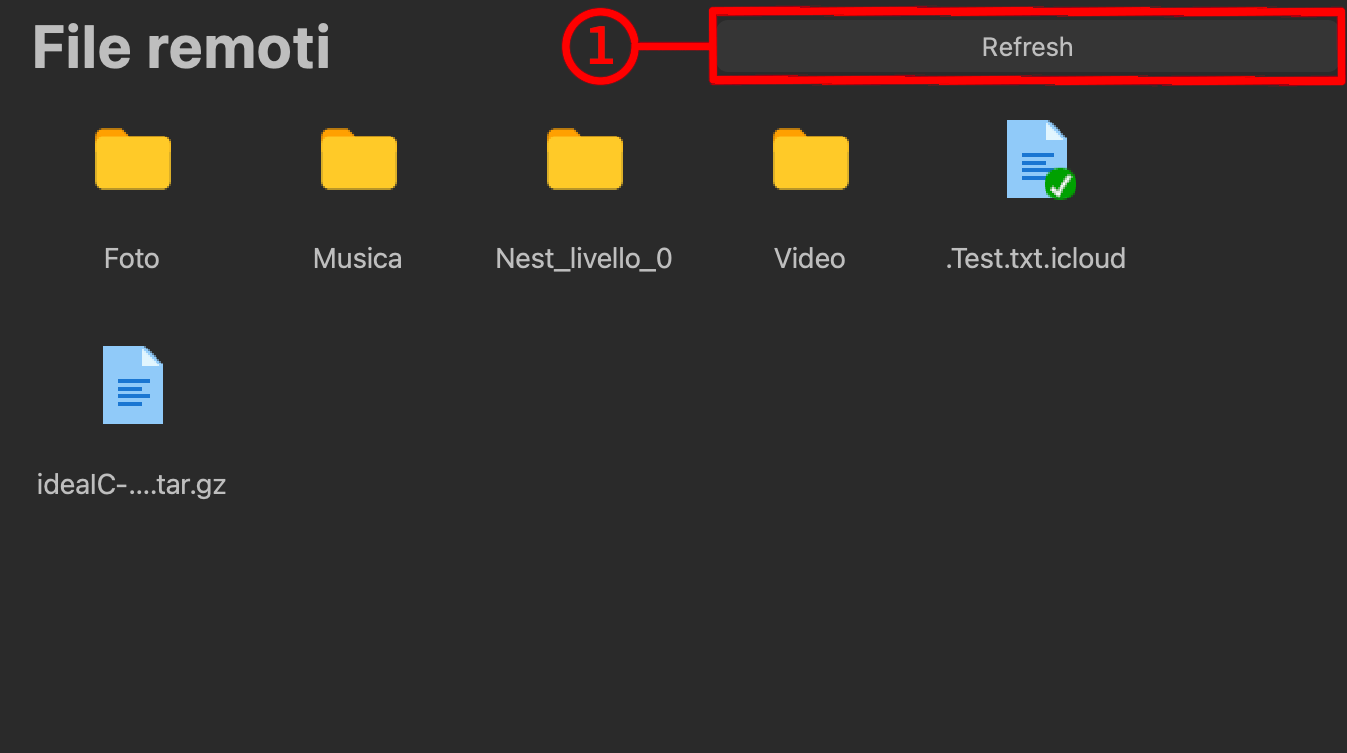
\includegraphics[scale = 0.8]{components/img/fileRem.png}
    \caption{Vista file remoti}
    \label{fig:fileRem}
\end{figure}
La vista si compone di una serie di icone che rappresentano i file o le cartelle presenti nella cartella remota. In alto a destra è presente un pulsante \textbf{[1]} che permette di effettuare il refresh della cartella remota.

\subsection{Icone di sincronizzazione}
\label{sec:iconeSync}
Per far sì che l'utente capisca a colpo d'occhio lo stato dei file ci sono tre icone che appariranno a seconda del caso in questione.
\subsubsection{Spunta su sfondo verde}

\begin{figure}[H]
    \centering
    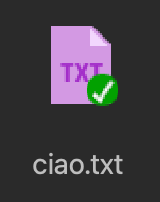
\includegraphics[scale = 0.8]{components/img/iconIsSync.png}
    \caption{Icona file sincronizzato}
    \label{fig:greenI}
\end{figure}

L'icona rappresentata in figura apparirà sui file presenti nella cartella locale e significa che il file è sincronizzato con il server.
\subsubsection{Frecce su sfondo blu}

\begin{figure}[H]
    \centering
    
\includegraphics[scale = 1.6]{components/img/iconSync.png}
    \caption{Icona file in sincronizzazione}
    \label{fig:bluedownI}
\end{figure}

L'icona rappresentata in figura apparirà sui file presenti nella cartella locale e significa che il file sta venendo sincronizzato con il server.

\subsubsection{Freccia verso il basso su sfondo blu}

\begin{figure}[H]
    \centering
    
\includegraphics[scale = 0.8]{components/img/iconUpdate.png}
    \caption{Icona file segnato da aggiornare}
    \label{fig:greenI}
\end{figure}


L'icona rappresentata in figura apparirà sui file presenti nella cartella remota e significa che quel file verrà aggiornato ogni volta che nel server sono presenti delle modifiche.

\subsection{Operazioni comuni}
In questa sezione vengono elencati i passaggi necessari per eseguire le operazioni più comuni previste dal programma.
\subsubsection{Scaricare un file dal server}
\begin{itemize}
\item Attivare la sincronizzazione cliccando il pulsante di sincronizzazione (\ref{fig:PsyncD});
\item Cliccare sul pulsante per visualizzare i file remoti (\ref{fig:PfileRem});
\item Navigare fino al file desiderato ed eseguire un click destro su di esso, quindi selezionare la voce "aggiungi a sync" dal menu contestuale;
\item Il file verrà sincronizzato allo scadere dell'intervallo di tempo di sincronizzazione selezionato, nel caso si volesse sincronizzare immediatamente il file è necessario cliccare sul pulsante per visualizzare i file sincronizzati (\ref{fig:PfileSync}) e cliccare sul pulsante "sincronizza ora".
\end{itemize}
\subsubsection{Eliminare un file dal server}
\begin{itemize}
\item Attivare la sincronizzazione cliccando il pulsante di sincronizzazione (\ref{fig:PsyncD});
\item Cliccare sul pulsante per visualizzare i file sincronizzati (\ref{fig:PfileSync});
\item Cliccare il pulsante "apri file manager";
\item Eliminare il file desiderato dal file manager;
\item Premere il pulsante "sincronizza ora" per aggiornare il server con i file locali, eliminando quindi il file eliminato in locale dal server.
\end{itemize}
\subsubsection{Rimuovere un file dalla sincronizzazione}
\begin{itemize}
\item Cliccare sul pulsante per visualizzare i file remoti (\ref{fig:PfileRem});
\item Navigare fino al file sincronizzato desiderato ed eseguire un click destro su di esso, quindi selezionare la voce "rimuovi da sync" dal menu contestuale. Il file verrà conservato in locale ma gli aggiornamenti ad esso non verranno più sincronizzati con il server e viceversa.
\end{itemize}

\subsection{Azioni sui file}
\label{sec:fileActions}

\subsubsection{Doppio click su un file}
Eseguendo un doppio click su un file nella vista File locali (\ref{sec:fileLocali}) il file verrà aperto dall'applicazione designata dal sistema.
\subsubsection{Click destro su un file}
Eseguendo un click destro su un file nella vista File remoti (\ref{sec:fileRemoti}) è possibile aggiungere o rimuovere un file dalla lista di sincronizzazione.  
\subsubsection{Doppio click su una cartella}
Eseguendo un doppio click su di una cartella, sia nella vista File locali che in quella File remoti, si scenderà di un livello, visualizzando il contenuto della cartella selezionata.
\subsubsection{Inserire file nella cartella locale}
Per inserire file nella cartella locale è necessario aprire il file manager utilizzando l'apposito pulsante e aggiungere file da esso.
\subsubsection{Refresh del server}
Per aggiornare la lista dei file visualizzati nella vista \ref{sec:fileRemoti} con le ultime modifiche avvenute nel server bisogna premere il pulsante "Refresh".
\subsubsection{Modifica di un file sincronizzato}
La modifica di un file sincronizzato avviene in maniera analoga alla modifica di un qualsiasi file locale, dopo aver effettuato i cambiamenti necessari è sufficiente salvare il documento e questo verrà automaticamente sincronizzato con il server.
\subsubsection{Cancellazione di un file sincronizzato}
L'eliminazione di un file sincronizzato avviene analogamente all'eliminazione di un qualsiasi file locale, dopo aver eliminato il file dalla cartella sincronizzata questa modifica verrà propagata anche sul server.

\subsection{Notifiche}
L'applicazione può inviare all'utente le seguenti notifiche:
\begin{itemize}
    \item Uno o più file sono stati scaricati;
    \item Uno o più file sono stati aggiornati;
    \item L'applicazione non è in grado di connettersi ad internet;
    \item L'utente ha esaurito la quota disco, quindi i file non possono essere scaricati;
    \item Le credenziali sono state cambiate, l'utente deve aggiornarle all'interno dell'applicazione.
\end{itemize}
Le notifiche che l'utente vedrà più spesso sono quelle relative ai file aggiornati e scaricati.
\begin{figure}[H]
    \centering
    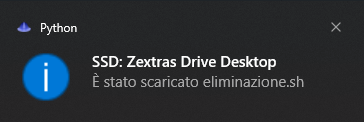
\includegraphics[scale = 0.7]{components/img/notifica_download_new_file.png}
    \caption{Notifica di un nuovo file che è stato scaricato}
    \label{fig:impostazioni}
\end{figure}
\begin{figure}[H]
    \centering
    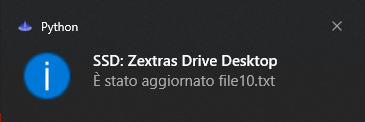
\includegraphics[scale = 0.7]{components/img/notifica_download_update_file.png}
    \caption{Notifica di un file che è stato aggiornato}
    \label{fig:impostazioni}
\end{figure}

\subsection{Impostazioni}
\label{sec:impostazioni}
\begin{figure}[H]
    \centering
    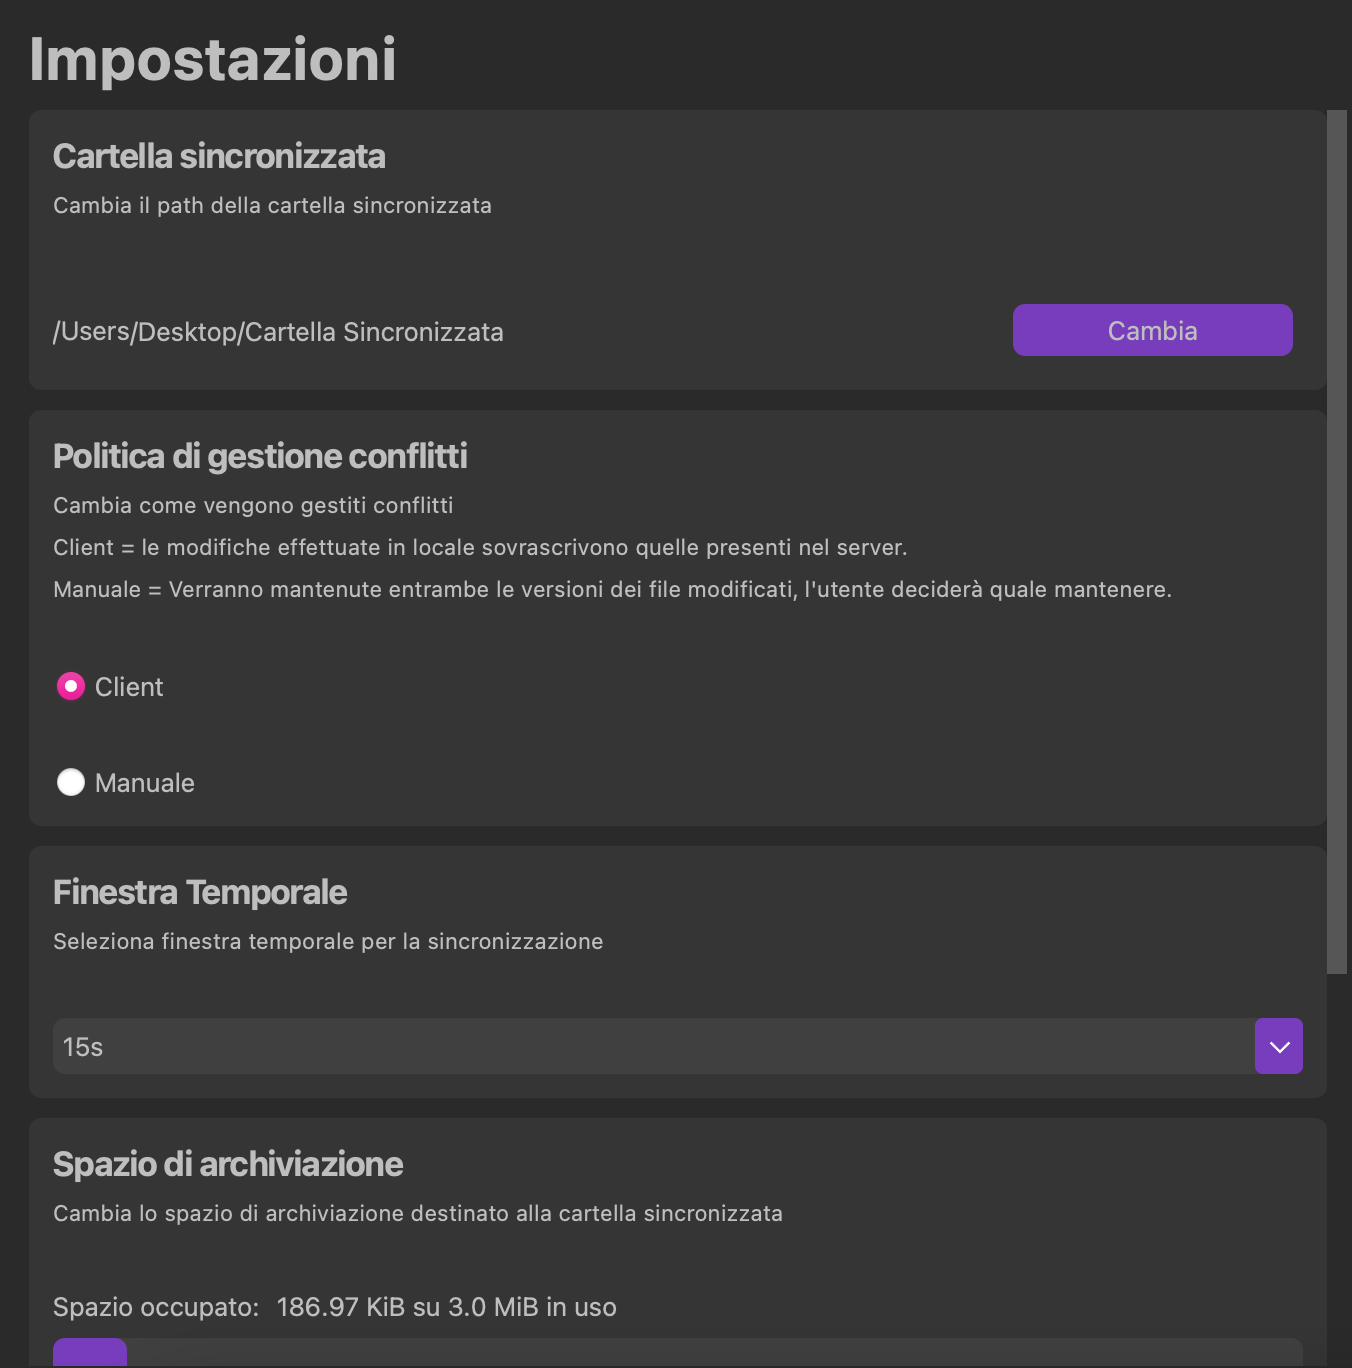
\includegraphics[scale = 0.7]{components/img/vistaImp.png}
    \caption{Vista impostazioni}
    \label{fig:impostazioni}
\end{figure}
La vista mostra una serie di riquadri con i quali è possibile interagire per modificare le impostazioni legate al software. Tramite l'apposita barra posizionata sulla destra è possibile visualizzare l'intera pagina delle impostazioni.

\subsubsection{Modifica path cartella}
\label{sec:cartella}
\begin{figure}[H]
    \centering
    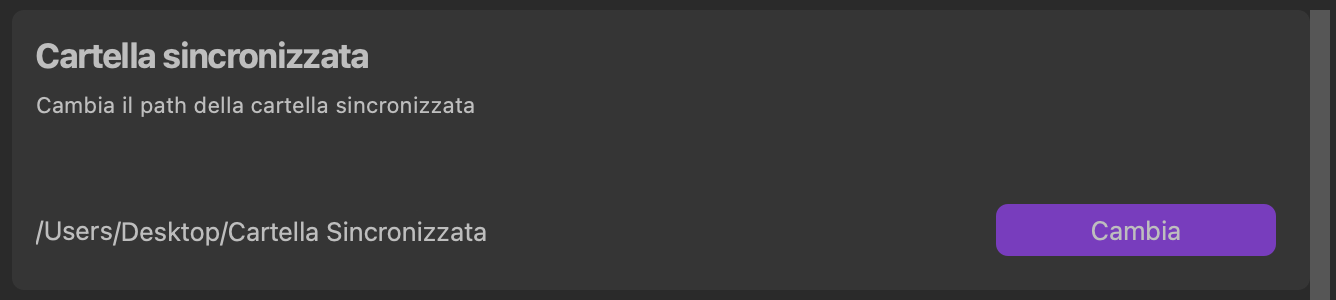
\includegraphics[scale = 1]{components/img/ImpCartella.png}
    \caption{Modifica percorso cartella}
    \label{fig:cartella}
\end{figure}
In questa sezione delle impostazioni è possibile modificare il percorso della cartella sincronizzata. Premendo il pulsante "Cambia" si aprirà una finestra che permetterà di cambiare il percorso (\S{}\ref{sec:selezionepath}).

\subsubsection{Modifica policy}
\label{sec:policy}
\begin{figure}[H]
    \centering
    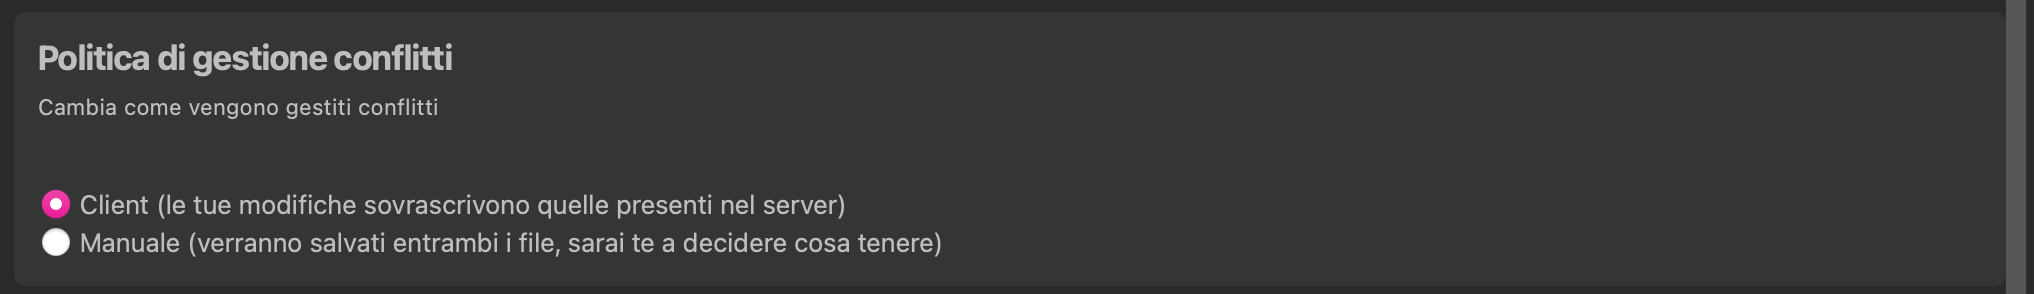
\includegraphics[scale = 0.4]{components/img/ImpPolicy.png}
    \caption{Modifica politica di risoluzione conflitti}
    \label{fig:policy}
\end{figure}
In questa sezione è possibile scegliere la politica di risoluzione dei conflitti. Ci sono due opzioni:
\begin{itemize}
\item\textbf{Client:} selezionando questa opzione le modifiche effettuate in locale andranno a sovrascrivere quelle caricate sul server;\
\item\textbf{Manuale:} selezionando questa opzione, ogni volta che il file in locale differisce dal file presente sul server verranno salvate entrambe le versioni in locale e sarà l'utente a decidere quale mantenere.\
\end{itemize}

\subsubsection{Modifica finestra temporale}
\label{sec:finestra temporale}
\begin{figure}[H]
    \centering
    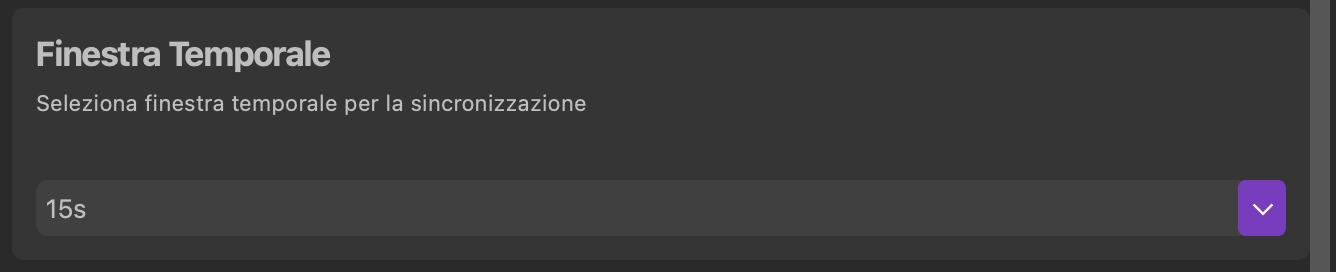
\includegraphics[scale = 0.65]{components/img/ImpFinTempA.png}
    \caption{Modifica finestra temporale}
    \label{fig:finTempA}
\end{figure}
In questa sezione è possibile modificare ogni quanto tempo avviare la sincronizzazione dal server alla cartella condivisa. Cliccando sull'apposita freccia a destra (Fig. \ref{fig:finTempC}) apparirà un elenco di possibili finestre temporali. 
\begin{figure}[H]
    \centering
    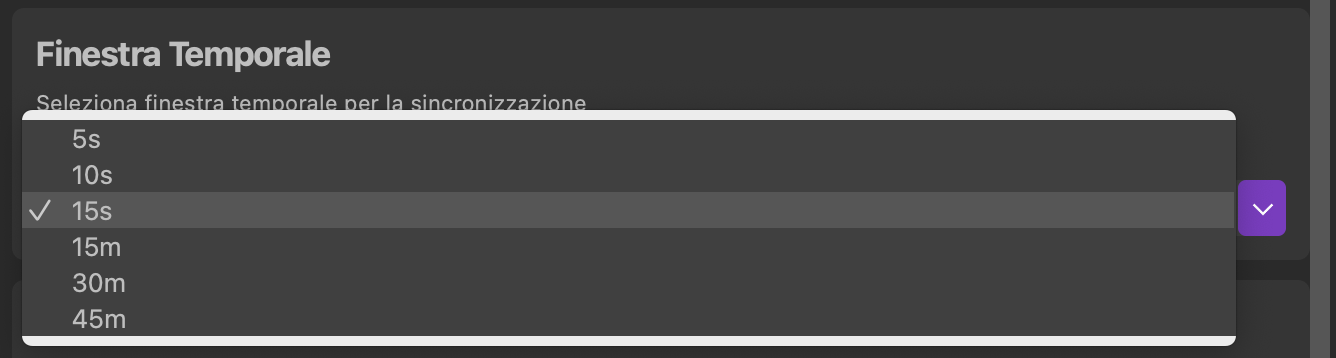
\includegraphics[scale = 0.65]{components/img/ImpFinTempC.png}
    \caption{Vista dopo aver cliccato sulla freccia}
    \label{fig:finTempC}
\end{figure}

\subsubsection{Modifica spazio di archiviazione}
\label{sec:quota}
\begin{figure}[H]
    \centering
    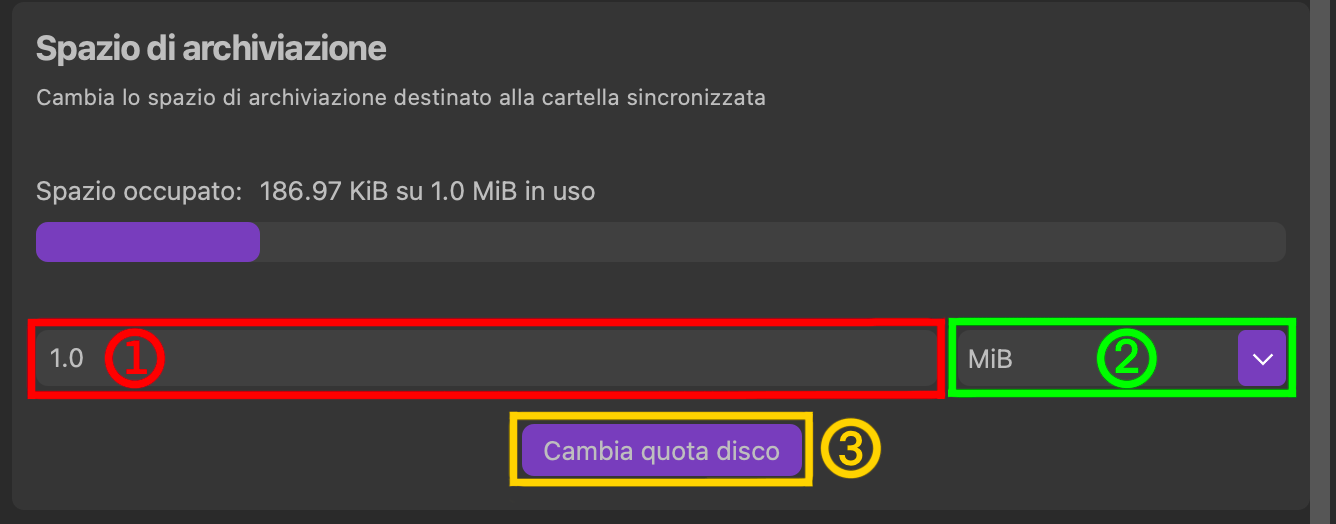
\includegraphics[scale = 0.8]{components/img/ImpQuota.png}
    \caption{Modifica quota disco}
    \label{fig:quota}
\end{figure}
In questa sezione è possibile modificare lo spazio di archiviazione dedicato alla cartella locale. In particolare, seguendo i numeri in Fig. \ref{fig:quota}:
\begin{enumerate}
\item permette di scrivere quanto spazio far occupare alla cartella;\
\item permette di decidere l'estensione del numero scritto (Fig. \ref{fig:quotazoom});\
\item pulsante che modifica lo spazio di archiviazione.\
\end{enumerate}
\begin{figure}[H]
    \centering
    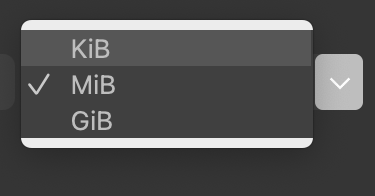
\includegraphics[scale = 1]{components/img/ImpQuota2.png}
    \caption{Vista dopo aver cliccato sulla freccia}
    \label{fig:quotazoom}
\end{figure}


\subsubsection{Profilo}
\label{sec:profilo}
\begin{figure}[H]
    \centering
    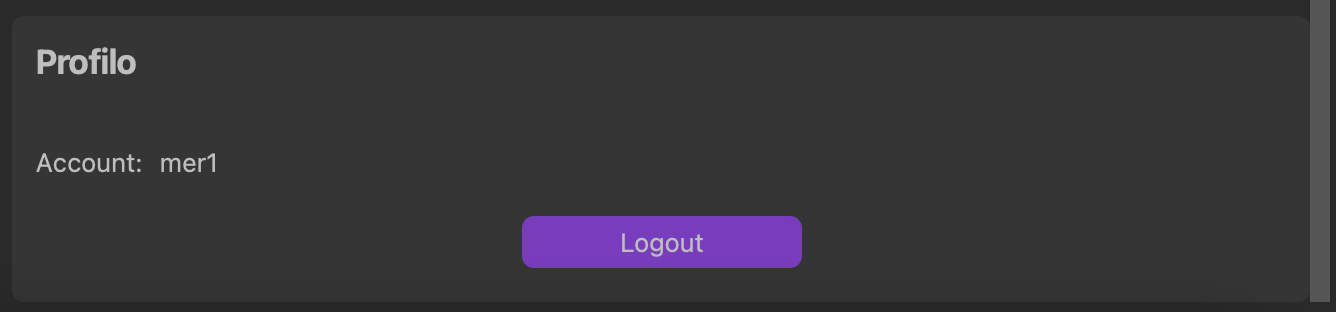
\includegraphics[scale = 0.65]{components/img/ImpLogout.png}
    \caption{Vista logout}
    \label{fig:fileRem}
\end{figure}
In questa sezione è possibile visualizzare il profilo collegato alle credenziali inserite. Inoltre, premendo il pulsante "Logout", è possibile disconnettere il profilo dal software: quest'ultimo si chiuderà e, al prossimo avvio, mostrerà la schermata di login (\S{}\ref{sec:autenticazione})


\newpage
\appendix

\section{Glossario} \label{sec:Glossario}
\subsubsection*{B}
\begin{itemize}
	\item \textbf{Bug}: Un problema che porta al malfunzionamento del software, tipicamente dovuto a un errore nella scrittura del codice sorgente di un programma.
\end{itemize}

\subsubsection*{C}
\begin{itemize}
	\item \textbf{Client}: Un qualunque componente software che accede ai servizi o alle risorse di un'altra componente detta server.
	\item \textbf{Cloud}: Indica un paradigma di erogazione di servizi offerti su richiesta da un fornitore a un cliente finale attraverso la rete internet, a partire da un insieme di risorse preesistenti, configurabili e disponibili in remoto sotto forma di architettura distribuita. 
	\item \textbf{Conflitto}: Si definisce conflitto tra due file se essi hanno lo stesso nome ed estensione risultando però diversi nel contenuto.
\end{itemize}
\subsubsection*{G}
\begin{itemize}
	\item \textbf{GitHub}: è un servizio di hosting per progetti software. Il nome "GitHub" deriva dal fatto che GitHub è una implementazione dello strumento di controllo versione distribuito Git.
\end{itemize}
\subsubsection*{H}
\begin{itemize}
	\item \textbf{Hardware}: Parte materiale di un sistema elettronico di elaborazione.
\end{itemize}

\subsubsection*{P}
\begin{itemize}
	\item \textbf{Python}: Linguaggio di programmazione orientato agli oggetti ad alto livello.
\end{itemize}

\subsubsection*{R}
\begin{itemize}
	\item \textbf{Repository}: Archivio digitale dove dati e informazioni sono raccolti, valorizzati e archiviati sulla base di metadati che ne permettono la rapida individuazione. Grazie alla sua peculiare architettura, un repository consente di gestire in modo ottimale anche grandi volumi di dati.
	\item \textbf{Requisiti minimi di sistema}: I requisiti sono le capacità minime sia hardware che software che il sistema dovrà avere per svolgere le funzioni.
\end{itemize}

\subsubsection*{S}
\begin{itemize}
	\item \textbf{Server}: Un componente che fornisce un servizio ad altre componenti chiamate client.
	\item \textbf{Software}: Insieme delle componenti immateriali di un sistema elettronico di elaborazione.
	\item \textbf{Solido}: In informatica, e in particolare in programmazione, l'acronimo SOLID si riferisce ai "primi cinque principi" dello sviluppo del software orientato agli oggetti descritti da Robert C. Martin in diverse pubblicazioni. I SOLID principles (Single responsibility, Open-closed, Liskov substitution, Interface segregation, Dependency inversion) sono intesi come linee guida per lo sviluppo di software leggibile, estendibile e mantenibile, in particolare nel contesto di pratiche di sviluppo agili.
	\item \textbf{SSD}: È l'acronimo di Soluzioni di Sincronizzazione Desktop. Il progetto didattico è stato presentato nel capitolato C7 del corso di Ingegneria del Software tenuto all'Università di Padova nel Corso di Laurea in Informatica dell'anno 2020/2021.
	\item \textbf{Sync engine}: È il software che opera nel computer, che confronta i file presenti nel computer e nel drive. Si occupa inoltre di decidere che operazioni fare con il server come il download o upload dei file.
\end{itemize}

\subsubsection*{Z}
\begin{itemize}
	\item \textbf{Zextras Drive}: Un nuovo componente di Zimbra che offre un sistema di archiviazione integrato con il WebClient di Zimbra. 
	\item \textbf{Zimbra}: Una suite di software collaborativi che include sia un server email che un web client.
\end{itemize}
\appendix
\newpage
\end{document}